% Options for packages loaded elsewhere
% Options for packages loaded elsewhere
\PassOptionsToPackage{unicode}{hyperref}
\PassOptionsToPackage{hyphens}{url}
%
\documentclass[
  11pt,
  letterpaper,
  DIV=11,
  numbers=noendperiod,
  twoside]{scrartcl}
\usepackage{xcolor}
\usepackage[left=1.1in, right=1in, top=0.8in, bottom=0.8in,
paperheight=9.5in, paperwidth=7in, includemp=TRUE, marginparwidth=0in,
marginparsep=0in]{geometry}
\usepackage{amsmath,amssymb}
\setcounter{secnumdepth}{3}
\usepackage{iftex}
\ifPDFTeX
  \usepackage[T1]{fontenc}
  \usepackage[utf8]{inputenc}
  \usepackage{textcomp} % provide euro and other symbols
\else % if luatex or xetex
  \usepackage{unicode-math} % this also loads fontspec
  \defaultfontfeatures{Scale=MatchLowercase}
  \defaultfontfeatures[\rmfamily]{Ligatures=TeX,Scale=1}
\fi
\usepackage{lmodern}
\ifPDFTeX\else
  % xetex/luatex font selection
  \setmathfont[]{Garamond-Math}
\fi
% Use upquote if available, for straight quotes in verbatim environments
\IfFileExists{upquote.sty}{\usepackage{upquote}}{}
\IfFileExists{microtype.sty}{% use microtype if available
  \usepackage[]{microtype}
  \UseMicrotypeSet[protrusion]{basicmath} % disable protrusion for tt fonts
}{}
\usepackage{setspace}
% Make \paragraph and \subparagraph free-standing
\makeatletter
\ifx\paragraph\undefined\else
  \let\oldparagraph\paragraph
  \renewcommand{\paragraph}{
    \@ifstar
      \xxxParagraphStar
      \xxxParagraphNoStar
  }
  \newcommand{\xxxParagraphStar}[1]{\oldparagraph*{#1}\mbox{}}
  \newcommand{\xxxParagraphNoStar}[1]{\oldparagraph{#1}\mbox{}}
\fi
\ifx\subparagraph\undefined\else
  \let\oldsubparagraph\subparagraph
  \renewcommand{\subparagraph}{
    \@ifstar
      \xxxSubParagraphStar
      \xxxSubParagraphNoStar
  }
  \newcommand{\xxxSubParagraphStar}[1]{\oldsubparagraph*{#1}\mbox{}}
  \newcommand{\xxxSubParagraphNoStar}[1]{\oldsubparagraph{#1}\mbox{}}
\fi
\makeatother


\usepackage{longtable,booktabs,array}
\usepackage{calc} % for calculating minipage widths
% Correct order of tables after \paragraph or \subparagraph
\usepackage{etoolbox}
\makeatletter
\patchcmd\longtable{\par}{\if@noskipsec\mbox{}\fi\par}{}{}
\makeatother
% Allow footnotes in longtable head/foot
\IfFileExists{footnotehyper.sty}{\usepackage{footnotehyper}}{\usepackage{footnote}}
\makesavenoteenv{longtable}
\usepackage{graphicx}
\makeatletter
\newsavebox\pandoc@box
\newcommand*\pandocbounded[1]{% scales image to fit in text height/width
  \sbox\pandoc@box{#1}%
  \Gscale@div\@tempa{\textheight}{\dimexpr\ht\pandoc@box+\dp\pandoc@box\relax}%
  \Gscale@div\@tempb{\linewidth}{\wd\pandoc@box}%
  \ifdim\@tempb\p@<\@tempa\p@\let\@tempa\@tempb\fi% select the smaller of both
  \ifdim\@tempa\p@<\p@\scalebox{\@tempa}{\usebox\pandoc@box}%
  \else\usebox{\pandoc@box}%
  \fi%
}
% Set default figure placement to htbp
\def\fps@figure{htbp}
\makeatother


% definitions for citeproc citations
\NewDocumentCommand\citeproctext{}{}
\NewDocumentCommand\citeproc{mm}{%
  \begingroup\def\citeproctext{#2}\cite{#1}\endgroup}
\makeatletter
 % allow citations to break across lines
 \let\@cite@ofmt\@firstofone
 % avoid brackets around text for \cite:
 \def\@biblabel#1{}
 \def\@cite#1#2{{#1\if@tempswa , #2\fi}}
\makeatother
\newlength{\cslhangindent}
\setlength{\cslhangindent}{1.5em}
\newlength{\csllabelwidth}
\setlength{\csllabelwidth}{3em}
\newenvironment{CSLReferences}[2] % #1 hanging-indent, #2 entry-spacing
 {\begin{list}{}{%
  \setlength{\itemindent}{0pt}
  \setlength{\leftmargin}{0pt}
  \setlength{\parsep}{0pt}
  % turn on hanging indent if param 1 is 1
  \ifodd #1
   \setlength{\leftmargin}{\cslhangindent}
   \setlength{\itemindent}{-1\cslhangindent}
  \fi
  % set entry spacing
  \setlength{\itemsep}{#2\baselineskip}}}
 {\end{list}}
\usepackage{calc}
\newcommand{\CSLBlock}[1]{\hfill\break\parbox[t]{\linewidth}{\strut\ignorespaces#1\strut}}
\newcommand{\CSLLeftMargin}[1]{\parbox[t]{\csllabelwidth}{\strut#1\strut}}
\newcommand{\CSLRightInline}[1]{\parbox[t]{\linewidth - \csllabelwidth}{\strut#1\strut}}
\newcommand{\CSLIndent}[1]{\hspace{\cslhangindent}#1}



\setlength{\emergencystretch}{3em} % prevent overfull lines

\providecommand{\tightlist}{%
  \setlength{\itemsep}{0pt}\setlength{\parskip}{0pt}}



 


\setlength\heavyrulewidth{0ex}
\setlength\lightrulewidth{0ex}
\usepackage[automark]{scrlayer-scrpage}
\clearpairofpagestyles
\cehead{
  Brian Weatherson
  }
\cohead{
  Why Ain’t Evidentialists Rich?
  }
\ohead{\bfseries \pagemark}
\cfoot{}
\makeatletter
\newcommand*\NoIndentAfterEnv[1]{%
  \AfterEndEnvironment{#1}{\par\@afterindentfalse\@afterheading}}
\makeatother
\NoIndentAfterEnv{itemize}
\NoIndentAfterEnv{enumerate}
\NoIndentAfterEnv{description}
\NoIndentAfterEnv{quote}
\NoIndentAfterEnv{equation}
\NoIndentAfterEnv{longtable}
\NoIndentAfterEnv{abstract}
\renewenvironment{abstract}
 {\vspace{-1.25cm}
 \quotation\small\noindent\emph{Abstract}:}
 {\endquotation}
\newfontfamily\tfont{EB Garamond}
\addtokomafont{disposition}{\rmfamily}
\addtokomafont{title}{\normalfont\itshape}
\let\footnoterule\relax

\makeatletter
\renewcommand{\@maketitle}{%
  \newpage
  \null
  \vskip 2em%
  \begin{center}%
  \let \footnote \thanks
    {\itshape\huge\@title \par}%
    \vskip 0.5em%  % Reduced from default
    {\large
      \lineskip 0.3em%  % Reduced from default 0.5em
      \begin{tabular}[t]{c}%
        \@author
      \end{tabular}\par}%
    \vskip 0.5em%  % Reduced from default
    {\large \@date}%
  \end{center}%
  \par
  }
\makeatother
\RequirePackage{lettrine}

\renewenvironment{abstract}
 {\quotation\small\noindent\emph{Abstract}:}
 {\endquotation\vspace{-0.02cm}}

\setmainfont{EB Garamond Math}[
  BoldFont = {EB Garamond SemiBold},
  ItalicFont = {EB Garamond Italic},
  RawFeature = {+smcp},
]

\newfontfamily\scfont{EB Garamond Regular}[RawFeature=+smcp]
\renewcommand{\textsc}[1]{{\scfont #1}}

\renewcommand{\LettrineTextFont}{\scfont}
\KOMAoption{captions}{tableheading}
\makeatletter
\@ifpackageloaded{caption}{}{\usepackage{caption}}
\AtBeginDocument{%
\ifdefined\contentsname
  \renewcommand*\contentsname{Table of contents}
\else
  \newcommand\contentsname{Table of contents}
\fi
\ifdefined\listfigurename
  \renewcommand*\listfigurename{List of Figures}
\else
  \newcommand\listfigurename{List of Figures}
\fi
\ifdefined\listtablename
  \renewcommand*\listtablename{List of Tables}
\else
  \newcommand\listtablename{List of Tables}
\fi
\ifdefined\figurename
  \renewcommand*\figurename{Figure}
\else
  \newcommand\figurename{Figure}
\fi
\ifdefined\tablename
  \renewcommand*\tablename{Table}
\else
  \newcommand\tablename{Table}
\fi
}
\@ifpackageloaded{float}{}{\usepackage{float}}
\floatstyle{ruled}
\@ifundefined{c@chapter}{\newfloat{codelisting}{h}{lop}}{\newfloat{codelisting}{h}{lop}[chapter]}
\floatname{codelisting}{Listing}
\newcommand*\listoflistings{\listof{codelisting}{List of Listings}}
\makeatother
\makeatletter
\makeatother
\makeatletter
\@ifpackageloaded{caption}{}{\usepackage{caption}}
\@ifpackageloaded{subcaption}{}{\usepackage{subcaption}}
\makeatother
\usepackage{bookmark}
\IfFileExists{xurl.sty}{\usepackage{xurl}}{} % add URL line breaks if available
\urlstyle{same}
\hypersetup{
  pdftitle={Why Ain't Evidentialists Rich?},
  pdfauthor={Brian Weatherson},
  hidelinks,
  pdfcreator={LaTeX via pandoc}}


\title{Why Ain't Evidentialists Rich?}
\author{Brian Weatherson}
\date{2024}
\begin{document}
\maketitle
\begin{abstract}
A common argument for favouring Evidential Decision Theory (EDT) over
Causal Decision Theory (CDT) is that EDT has predictably higher expected
returns in Newcomb Problems. But this doesn't show much. For almost any
pair of theories you can come up with cases where one does, on average,
better than the other. Here I describe a case involving dynamic choice
where EDT predictably does worse than CDT. (This paper is forthcoming in
\emph{Analysis}.)
\end{abstract}


\setstretch{1.1}
There is a familiar complaint against Causal Decision Theory (CDT) that
goes back to the modern origins of decision theory in the 1970s. Here is
a recent version of it due to Ahmed and Price
(\citeproc{ref-AhmedPrice2012}{2012}). (I've slightly changed some of
the wording, but otherwise this argument is quoted from page 16 of their
paper.)

\begin{enumerate}
\def\labelenumi{\arabic{enumi}.}
\tightlist
\item
  In Newcomb problems, the average returns to one-boxing exceed that to
  two-boxing.
\item
  Everyone can see that (1) is true.
\item
  Therefore one-boxing foreseeably does better than two-boxing. (by 1,
  2)
\item
  Therefore Causal Decision Theory (CDT) is committed to the foreseeably
  worse option for anyone facing Newcomb's problem.
\end{enumerate}

Here's what they, and many other proponents of Evidential Decision
Theory (EDT) say follows from 4.

\begin{quote}
The point of the argument is that if everyone knows that the
CDT-irrational strategy will in fact do better on average than the
CDT-rational strategy, then it's rational to play the CDT-irrational
strategy. (\citeproc{ref-AhmedPrice2012}{Ahmed and Price 2012, 17})
\end{quote}

This is what Lewis (\citeproc{ref-Lewis1981en}{1981b}) called the ``Why
Ain'cha Rich'' argument, and what following Ahmed
(\citeproc{ref-Ahmed2014}{2014, 182}) and Bales
(\citeproc{ref-Bales2018}{2018}) I'll call the WAR argument. I'm going
to argue the last step of the WAR argument doesn't follow. Or, more
precisely, that proponents of EDT cannot coherently say that it follows.
For there are cases where EDT foreseeably does worse than at least some
prominent versions of CDT.\footnote{Ian Wells
  (\citeproc{ref-Wells2019}{2019}) has another case where EDT does worse
  than some versions of CDT. I think his case successfully shows that
  WAR arguments are no good, but not everyone is convinced. I'll come
  back to Wells's case in Section~\ref{sec-wells-ahmed}.}

\section{Coins and Signals}\label{sec-coinssignals}

The example I'll use is a version of a signalling game of the kind
introduced by Lewis (\citeproc{ref-Lewis1969a}{1969}). And in particular
it's a version of the broadly adversarial kind of signalling game that
is central to the plot of Cho and Kreps
(\citeproc{ref-ChoKreps1987}{1987}). It will involve a human Chooser,
and a Demon who is excellent at predictions. The game will have three
stages.

At the first stage a fair coin is flipped, and the result shown to
Chooser, but not to Demon. At the second stage, Chooser will choose Up
or Down, and the choice will be publicly announced. At the third stage,
Demon will try to guess what the coin showed. Demon knows the payoff
table I'm about to show you, and is arbitrarily good at predicting
Chooser's strategy for what to do given how the coin appears. This
prediction is causally independent of Chooser's choice, but Demon's
guess is not independent; it could be affected by the choice. The
payoffs to each player are a function of what happens at each of the
three steps, and are given by table Table~\ref{tbl-payoffs-demon-coin}.
(The payoffs here are all in utils.)

\begin{longtable}[]{@{}
  >{\centering\arraybackslash}p{(\linewidth - 8\tabcolsep) * \real{0.1389}}
  >{\centering\arraybackslash}p{(\linewidth - 8\tabcolsep) * \real{0.1806}}
  >{\centering\arraybackslash}p{(\linewidth - 8\tabcolsep) * \real{0.1528}}
  >{\centering\arraybackslash}p{(\linewidth - 8\tabcolsep) * \real{0.2778}}
  >{\centering\arraybackslash}p{(\linewidth - 8\tabcolsep) * \real{0.2500}}@{}}
\caption{Payouts for the coins and signals
game}\label{tbl-payoffs-demon-coin}\tabularnewline
\toprule\noalign{}
\begin{minipage}[b]{\linewidth}\centering
\textbf{Coin}
\end{minipage} & \begin{minipage}[b]{\linewidth}\centering
\textbf{Chooser}
\end{minipage} & \begin{minipage}[b]{\linewidth}\centering
\textbf{Demon}
\end{minipage} & \begin{minipage}[b]{\linewidth}\centering
\textbf{Chooser Payoff}
\end{minipage} & \begin{minipage}[b]{\linewidth}\centering
\textbf{Demon Payoff}
\end{minipage} \\
\midrule\noalign{}
\endfirsthead
\toprule\noalign{}
\begin{minipage}[b]{\linewidth}\centering
\textbf{Coin}
\end{minipage} & \begin{minipage}[b]{\linewidth}\centering
\textbf{Chooser}
\end{minipage} & \begin{minipage}[b]{\linewidth}\centering
\textbf{Demon}
\end{minipage} & \begin{minipage}[b]{\linewidth}\centering
\textbf{Chooser Payoff}
\end{minipage} & \begin{minipage}[b]{\linewidth}\centering
\textbf{Demon Payoff}
\end{minipage} \\
\midrule\noalign{}
\endhead
\bottomrule\noalign{}
\endlastfoot
H & U & H & 40 & 1 \\
H & U & T & 400 & 0 \\
H & D & H & 0 & 1 \\
H & D & T & 0 & 0 \\
T & U & H & 40 & 0 \\
T & U & T & 28 & 1 \\
T & D & H & 0 & 0 \\
T & D & T & 44 & 1 \\
\end{longtable}

Figure~\ref{fig-second-anti-war} shows the game they are playing in tree
form. We start at the middle, then move left or right depending on the
coin flip, up or down depending on Chooser's choice, and at one or other
angle depending on Demon's choice. Demons's payoffs are just as you'd
expect - they get rewarded iff they figure out how the coin landed.
Chooser's payoffs are more complicated, but the big things to note are
the huge payout if they get to the top-left and Demon does not make a
correct prediction, and the generally poor payouts for choosing Down.

\begin{figure}

\centering{

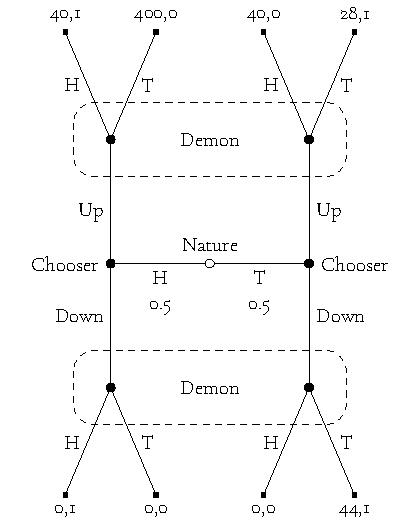
\includegraphics[width=0.8\linewidth,height=\textheight,keepaspectratio]{diagram.pdf}

}

\caption{\label{fig-second-anti-war}Tree Diagram of the Coins and
Signals Game}

\end{figure}%

I intend the Demon to be a rational player in a game-theoretic sense.
But to translate that into decision-theoretic terms, it's important to
make a few stipulations. Demon predicts Chooser's strategy, that is
Chooser's plan about what to do if the coin lands Heads and what to do
if the coin lands Tails, before the game starts. They make their guess
about how the coin landed after seeing Chooser's actual choice, and
updating their prior beliefs (about both the coin and Chooser) with this
information. If they predict that Chooser will do the same thing however
the coin lands, they will have no useful information about the coin, so
they will flip their own coin to make a guess. In that case it will be
50/50 whether Demon says Heads or Tails. Also, if Demon is surprised by
what Chooser does, i.e., if they had predicted Chooser would do one
thing however the coin lands but Chooser does the other thing, Demon
will also flip their own coin to make a guess.\footnote{A key move Cho
  and Kreps (\citeproc{ref-ChoKreps1987}{1987}) is that in some cases we
  can say substantive things about what a player will do if they are
  surprised in this sense. But Figure~\ref{fig-second-anti-war} is not
  one of these cases.} Finally, Demon's predictions are arbitrarily
accurate. It makes the math easiest to assume Demon is correct with
probability 1. Some people (myself among them) worry that stipulating
the Demon succeeds with probability 1 might take us too close to a case
of backwards causation, and it's very important that Chooser does not
cause Demon's prediction of a strategy. If you have that worry, say that
Demon's probability of successful prediction (whichever of the four
strategies Chooser opts for) is 1~-~\(\varepsilon\), where
\(\varepsilon\) is small enough that it doesn't make a difference to
what is rational for Chooser to do.

Now I want to analyse what Chooser will do if they follow EDT. It should
be fairly clear that if the coin lands Heads, Chooser should say Up. The
worst possible return from Up is 40, the best possible return from Down
is 0. So playing Up if the coin lands Heads is what any theory would
recommend, and Chooser will do that whether or not they follow EDT.
Indeed, this is so clear that we should assume Demon will predict that
Chooser will play Up if the coin lands Heads. So what happens if the
coin lands Tails? There are four possibilities here: the two things
Chooser might do crossed with the two predictions Demon might make. The
expected return to Chooser in these four possibilities is given in
Table~\ref{tbl-payout-if-tails}.

\begin{longtable}[]{@{}ccc@{}}
\caption{The expected payout to Chooser in four cases if the coin lands
Tails}\label{tbl-payout-if-tails}\tabularnewline
\toprule\noalign{}
& \textbf{Predict Up} & \textbf{Predict Down} \\
\midrule\noalign{}
\endfirsthead
\toprule\noalign{}
& \textbf{Predict Up} & \textbf{Predict Down} \\
\midrule\noalign{}
\endhead
\bottomrule\noalign{}
\endlastfoot
\textbf{Up} & 34 & 40 \\
\textbf{Down} & 22 & 44 \\
\end{longtable}

The numbers in Table~\ref{tbl-payout-if-tails} aren't entirely obvious;
I'll spell out how I got them.

\begin{itemize}
\tightlist
\item
  If Demon predicts Up if Tails, Demon will flip a coin if the coin
  lands Tails, whatever Chooser does. That's because they'll either get
  no information (if Chooser plays Up), or will be surprised (if Chooser
  plays Down). So Chooser will get the average of lines 5 and 6 in
  Table~\ref{tbl-payoffs-demon-coin} if they play Up, and the average of
  lines 7 and 8 if they play Down.
\item
  If Demon predicts Down if Tails, and Chooser plays Up, Demon will
  think (falsely) that the coin must have landed Heads, since Demon will
  have predicted that Chooser will only say Up if Heads. So Demon will
  say Heads. So we'll definitely be at line 5 of
  Table~\ref{tbl-payoffs-demon-coin}, where Chooser gets 40.
\item
  If Demon predicts Down if Tails, and Chooser plays Down, Demon will
  think (correctly) that the coin must have landed Tails. So Demon will
  say that, and we'll be at line 8 of
  Table~\ref{tbl-payoffs-demon-coin}.
\end{itemize}

In a decision problem like Table~\ref{tbl-payout-if-tails}, EDT says
that if Demon is sufficiently likely to be accurate, all that matters is
which of the top-left and bottom-right cells is largest. In this case,
it's the bottom-right, so EDT says to play Down. That isn't absurd in
Table~\ref{tbl-payout-if-tails} itself; it almost certainly results in
Chooser getting the best possible payout of 44. So that's our analysis
of the game for EDT: Chooser plays Up if Heads, Down if Tails, gets 40
if Heads and 44 if Tails (plus/minus a small amount in expectation if
Demon has \(\varepsilon\) chance of being wrong), and on average gets
42. What does CDT say? This needs a small detour, because `CDT' has
become an ambiguous signifier.

\section{What is CDT?}\label{sec-cdt-definition}

David Lewis (\citeproc{ref-Lewis1981bn}{1981a}) argued that all
then-existing versions of CDT were little more than notational variants;
they just differed on ``emphasis and formulation''
(\citeproc{ref-Lewis1981bn}{Lewis 1981a, 5}). Whether that was true then
(and I have some doubts), it isn't true now. There are now many broadly
causal decision theories, i.e., theories that say one should take two
boxes in Newcomb's Problem because it is the causally dominant option,
on the philosophical market. To see the available variety, it helps to
consider a very abstract decision problem. Chooser has to choose Up or
Down, arbitrarily accurate Demon has predicted what Chooser will select,
and the payoffs are a function of the choice and the prediction.
Table~\ref{tbl-abstract} presents the abstract form of that problem.

\begin{longtable}[]{@{}ccc@{}}
\caption{An abstract decision
problem}\label{tbl-abstract}\tabularnewline
\toprule\noalign{}
& \textbf{Predict Up} & \textbf{Predict Down} \\
\midrule\noalign{}
\endfirsthead
\toprule\noalign{}
& \textbf{Predict Up} & \textbf{Predict Down} \\
\midrule\noalign{}
\endhead
\bottomrule\noalign{}
\endlastfoot
\textbf{Up} & \emph{a} & \emph{b} \\
\textbf{Down} & \emph{c} & \emph{d} \\
\end{longtable}

To make the analysis a little easier, I'm going to assume all four of
these values are distinct. We could get to the same conclusions as I
reach below without this assumption, but we'd have to spent a lot of
time checking edge cases. And I've set up the puzzles in this paper so
that questions about what to do if any of these values are equal don't
come up.

As noted in Section~\ref{sec-coinssignals}, if Demon is accurate enough,
EDT just cares about whether \emph{a} or \emph{d} is larger. What's
definitional of CDT is that if the prediction is causally independent of
the choice, and \emph{a}~\textgreater~\emph{c}, and
\emph{b}~\textgreater~\emph{d}, then Up is the right choice.\footnote{To
  be clear, \emph{I} am taking this to be definitional of being a causal
  decision theory. I think this is a fairly standard usage outside of
  decision theory, but not all decision theorists go along with it.} But
what if only one of those inequalities hold? In particular, if
\emph{a}~\textgreater~\emph{c}, and \emph{d}~\textgreater~\emph{b}, what
is to be done? There are, in the current literature, four different
verdicts on this among people who agree with the fundamental claim that
CDT makes about Newcomb-like problems.

\begin{enumerate}
\def\labelenumi{\arabic{enumi}.}
\tightlist
\item
  Frank Arntzenius (\citeproc{ref-Arntzenius2008}{2008}) and Johan
  Gustafsson (\citeproc{ref-Gustafsson2011}{2011}) say that in this case
  CDT should follow EDT, and use the values of \emph{a} and \emph{d} to
  settle the choice. In Table~\ref{tbl-payout-if-tails} that means
  playing Down, since 44~\textgreater~34.
\item
  Ralph Wedgwood (\citeproc{ref-Wedgwood2013a}{2013}), Dmitri Gallow
  (\citeproc{ref-Gallow2020}{2020}), Abelard Podgorski
  (\citeproc{ref-Podgorski2022}{2022}), and David Barnett
  (\citeproc{ref-Barnett2022}{2022}) say that Chooser should choose Up
  or Down depending on which of \emph{a} + \emph{b} and \emph{c} +
  \emph{d} is larger.\footnote{My description these four theories may
    seem surprising since they do not emphasise the comparison between
    \emph{a} +~\emph{b} and \emph{c} +~\emph{d}, but rather the
    comparison between \emph{a} -~\emph{c} and \emph{d} -~\emph{b}. This
    is just a notational variation, and I find my variant easier to use,
    if a little removed from the underlying philosophical motivation.}
  In Table~\ref{tbl-payout-if-tails} they recommend Up, since 34 +
  40~\textgreater~22 + 44.
\item
  Jack Spencer (\citeproc{ref-Spencer2023}{2023}) and Melissa Fusco
  (\citeproc{ref-Fuscond}{n.d.}) say that if
  \emph{a}~\textgreater~\emph{c}, and \emph{d}~\textgreater~\emph{b},
  either Up or Down is rationally permissible.
\item
  James Joyce (\citeproc{ref-Joyce2012}{2012}) says that what Chooser
  does if \emph{a}~\textgreater~\emph{c}, and
  \emph{d}~\textgreater~\emph{b} should be a function of how likely they
  think it is at the start of deliberation that they will choose Up or
  Down.
\end{enumerate}

So these four families of theories say different things about cases like
Table~\ref{tbl-payout-if-tails}. And within each family (except possibly
the last), it isn't hard to find other cases where the theories
disagree. The best conclusion, I think, is that there are Causal
Decision \emph{Theories}, but no one Causal Decision \emph{Theory}. CDT
is a name for a family of views, not a particular view. There are some
people in the literature who try to use the term for one particular one
of the nine views I just described\footnote{Or possibly for an older
  theory like the one defended by Gibbard and Harper
  (\citeproc{ref-GibbardHarper1978}{1978}) or the one defended by Lewis
  (\citeproc{ref-Lewis1981bn}{1981a})}, but I can't see what
particularly motivates any one choice; they all look equally deserving
of the term to me.

This is an asymmetry between EDT and CDT. EDT is indeed a theory; it is
the theory defended by Arif Ahmed (\citeproc{ref-Ahmed2014}{2014}). But
CDT is a family of theories. So we shouldn't compare EDT to CDT as such,
we should compare it to a particular causal theory. And for this paper,
I'll focus on the theories listed in point 2 above, and especially the
version defended by Gallow.

On Gallow's view, Chooser should play Up in
Table~\ref{tbl-payout-if-tails}, since 34 + 40~\textgreater~22 + 44. So
Chooser will always play Up in Figure~\ref{fig-second-anti-war}. So
Demon will always flip a coin to decide what to do. So all of the
outcomes where Chooser plays Up are equally likely.\footnote{That is,
  the four outcomes at the top of Figure~\ref{fig-second-anti-war}, or
  options 1, 2, 5, and 6 in Table~\ref{tbl-payoffs-demon-coin}.} That
means Chooser will on average get a return of 127. Since
127~\textgreater~42, on average if Chooser follows Gallow's theory they
will get a better return than if they follow EDT. So if WAR arguments
work, they show that EDT should be rejected since it does worse than
Gallow's theory in cases like
Figure~\ref{fig-second-anti-war}.\footnote{As a referee points out, this
  doesn't show that WAR arguments would give one a reason to
  \emph{endorse} Gallow's theory. After all, since Gallow's theory is a
  version of CDT, it has worse returns on average than EDT in Newcomb
  problems. The real point is that showing theory A has better returns
  than theory B in one particular problem doesn't mean much unless we
  show that there is no problem where theory B does better.}

\section{Wells and Ahmed}\label{sec-wells-ahmed}

Ian Wells (\citeproc{ref-Wells2019}{2019}) has earlier offered an
example where EDT predictably does worse than (all versions of) CDT. His
case involves a two-step game, where the EDTer will, at step 2, make a
decision that everyone, whether they believe in CDT or EDT or any other
plausible theory, think is bad from the perspective of the player at
step 1. At round 1 the players can pay to tie their hands at round 2,
and the EDTer will make this payment. (As would the CDTer who thinks
they will become an EDTer before round 2 starts.) Arif Ahmed
(\citeproc{ref-Ahmed2020}{2020}) responds that this is an unfair
criticism. In Wells's cases, he says, the EDT and CDT deciders are not
in equivalent situations in round one. The EDTer knows that they will
use EDT in later rounds, and the CDTer knows that they will use CDT in
later rounds. So they have different evidence about what will happen at
some later time in a way that's relevant to their current decision, so
it's not a like-for-like comparison between CDT and EDT at the first
stage.

The first thing to say is that I'm not sure this is a fair criticism of
Wells. If WAR arguments work anywhere (something that Ahmed believes but
Wells is only assuming for \emph{reductio}), they are meant to work
against CDT in Newcomb's Problem. But in that case the CDTer and EDTer
also have different subjective credences about the problem they face.
The CDTer thinks that they have a transparent box and an empty box in
front of them; the EDTer thinks that they have a transparent box and a
box full of money in front of them. If differences in credences about
what one will do mean that WAR arguments are unfair, then WAR arguments
don't work in the very case they are designed for. So I think Wells's
argument works, and that Ahmed's criticism does not rescue the argument
for EDT.

Set that aside though, because the main thing I want to add is that my
example does not turn on differences in the subjective states of the
possible choosers. Every chooser, whether they follow EDT, Gallow's
theory, or any other, will choose Up if the coin lands Heads. And this
is common knowledge. Demon knows this, and Chooser knows that Demon
knows it, and so on. The only difference is that if Chooser follows EDT,
they will play Down if Tails. And that's good as far as it goes; they'll
probably get the highest possible payoff they can get at that point.
More importantly for this debate, they will have the same subjective
states if Tails is true whether they follow EDT, Gallow's theory, or
anything else. They will believe that they would have played Up if
Heads, and that the Demon would have predicted that. So the different
choices they make if the coin lands Tails can't be traced back to
differences in their subjective states. So the complaint that Ahmed
makes about Wells's examples can't be made here (even setting aside the
question of whether it is a fair complaint). Nonetheless, the EDTer ends
up with less money in the long run than the follower of Gallow's theory
when playing this game.

\section{Why The Examples Matter}\label{why-the-examples-matter}

This paper is very much not an argument against EDT; instead, it's part
of a war on WAR. WAR arguments overgenerate. They sometimes `show' that
EDT is better than Gallow-style CDT, as in Newcomb's Problem, but
sometimes they `show' the reverse, as in
Figure~\ref{fig-second-anti-war}.

Even when they seem to favour a view like Gallow's, it's something of a
coincidence that they do. Go back to Table~\ref{tbl-payoffs-demon-coin},
and replace the payoff to Chooser at line 2 with a variable \emph{x}. As
long as \emph{x}~\textgreater~0, Gallow-style CDT will still say to
choose Up however the coin lands. The value of \emph{x} is irrelevant to
what to do if Tails, and as long as \emph{x}~\textgreater~0, Up is
guaranteed to do better than Down if the coin lands Heads. But if
\emph{x} \textless{} 60, the average payoff to EDT, which is 42 whatever
the value of \emph{x} is, will be greater than the average payoff to
Gallow-style CDT, which is (108~+~\emph{x})/4.

So which of these two theories is favoured by WAR considerations turns
on a factor, namely the value of \emph{x}, that's not part of the
decision process for either theory in the only part of the decision tree
where they differ. The two theories differ on what to do if the coin
lands Tails. And that turns entirely on the payouts in lines 5 to 8.
This is because both theories are consequentialist theories in the sense
of consequentialism popularised by Hammond
(\citeproc{ref-Hammond1988}{1988}). That's I think the deepest lesson of
this example. Which theory is favoured by WAR considerations is a deeply
non-consequentialist consideration; it's about what theory one would
have been best off adopting originally. So strange things can happen if
you use it to `decide' between competing consequentialist theories. What
the example reveals is that those strange things actually happen in some
specifiable cases.

Now I haven't said anything here about whether non-consequentialists can
legitimately use WAR arguments. And this matters a bit more than it used
to, because there are sophisticated defenders of non-consequentialism,
such as Levinstein and Soares
(\citeproc{ref-LevinsteinSoares2020}{2020}). Nothing I've said here
tells against the use of WAR arguments by such theories. I think there
are independent arguments against these non-consequentialist theories,
especially when one thinks about cases where generally reliable
predictors are known to have made mistakes, but that's a story for
another day. What I hope to have shown here is that proponents of EDT
cannot coherently use WAR arguments. And while I haven't proven this
generalises to all consequentialist theories, i.e., that no
consequentialist theory can coherently use WAR arguments, I think cases
like mine make that generalisation more probable.\footnote{Thanks to two
  very helpful reviewers for \emph{Analysis}, who corrected several
  mistakes in an earlier version of this paper, pushed me to clarify
  things that I'd rushed by (and at least in two cases made a clumsy
  error in the rush), and pointed out ways in which I needed to engage
  more with existing work. The comments helped every part of the paper,
  but in particular this conclusion about just what the cases show, and
  why they show that, owes a lot to their feedback.}

\subsection*{References}\label{references}
\addcontentsline{toc}{subsection}{References}

\phantomsection\label{refs}
\begin{CSLReferences}{1}{0}
\bibitem[\citeproctext]{ref-Ahmed2014}
Ahmed, Arif. 2014. \emph{Evidence, Decision and Causality}. Cambridge:
{C}ambridge {U}niversity {P}ress.

\bibitem[\citeproctext]{ref-Ahmed2020}
---------. 2020. {``Equal Opportunities in Newcomb's Problem and
Elsewhere.''} \emph{Mind} 129 (515): 867--86. doi:
\href{https://doi.org/10.1093/mind/fzz073}{10.1093/mind/fzz073}.

\bibitem[\citeproctext]{ref-AhmedPrice2012}
Ahmed, Arif, and Huw Price. 2012. {``Arntzenius on `Why Ain'cha
Rich?'.''} \emph{Erkenntnis} 77 (1): 15--30. doi:
\href{https://doi.org/10.1007/s10670-011-9355-2}{10.1007/s10670-011-9355-2}.

\bibitem[\citeproctext]{ref-Arntzenius2008}
Arntzenius, Frank. 2008. {``No Regrets; or, Edith Piaf Revamps Decision
Theory.''} \emph{Erkenntnis} 68 (2): 277--97. doi:
\href{https://doi.org/10.1007/s10670-007-9084-8}{10.1007/s10670-007-9084-8}.

\bibitem[\citeproctext]{ref-Bales2018}
Bales, Adam. 2018. {``Richness and Rationality: Causal Decision Theory
and the WAR Argument.''} \emph{Synthese} 195 (1): 259--67. doi:
\href{https://doi.org/10.1007/s11229-016-1214-x}{10.1007/s11229-016-1214-x}.

\bibitem[\citeproctext]{ref-Barnett2022}
Barnett, David James. 2022. {``Graded Ratifiability.''} \emph{Journal of
Philosophy} 119 (2): 57--88. doi:
\href{https://doi.org/10.5840/jphil202211925}{10.5840/jphil202211925}.

\bibitem[\citeproctext]{ref-ChoKreps1987}
Cho, In-Koo, and David M. Kreps. 1987. {``Signalling Games and Stable
Equilibria.''} \emph{The Quarterly Journal of Economics} 102 (2):
179--221. doi: \href{https://doi.org/10.2307/1885060}{10.2307/1885060}.

\bibitem[\citeproctext]{ref-Fuscond}
Fusco, Melissa. n.d. {``Absolution of a Causal Decision Theorist.''}
\emph{No{û}s}. doi:
\href{https://doi.org/10.1111/nous.12459}{10.1111/nous.12459}. Early
view.

\bibitem[\citeproctext]{ref-Gallow2020}
Gallow, J. Dmitri. 2020. {``The Causal Decision Theorist's Guide to
Managing the News.''} \emph{The Journal of Philosophy} 117 (3): 117--49.
doi:
\href{https://doi.org/10.5840/jphil202011739}{10.5840/jphil202011739}.

\bibitem[\citeproctext]{ref-GibbardHarper1978}
Gibbard, Allan, and William Harper. 1978. {``Counterfactuals and Two
Kinds of Expected Utility.''} In \emph{Foundations and Applications of
Decision Theory}, edited by C. A. Hooker, J. J. Leach, and E. F.
McClennen, 125--62. Dordrecht: Reidel.

\bibitem[\citeproctext]{ref-Gustafsson2011}
Gustafsson, Johan E. 2011. {``A Note in Defence of Ratificationism.''}
\emph{Erkenntnis} 75 (1): 147--50. doi:
\href{https://doi.org/10.1007/s10670-010-9267-6}{10.1007/s10670-010-9267-6}.

\bibitem[\citeproctext]{ref-Hammond1988}
Hammond, Peter J. 1988. {``Consequentialist Foundations for Expected
Utility.''} \emph{Theory and Decision} 25 (1): 25--78. doi:
\href{https://doi.org/10.1007/BF00129168}{10.1007/BF00129168}.

\bibitem[\citeproctext]{ref-Joyce2012}
Joyce, James M. 2012. {``Regret and Instability in Causal Decision
Theory.''} \emph{Synthese} 187 (1): 123--45. doi:
\href{https://doi.org/10.1007/s11229-011-0022-6}{10.1007/s11229-011-0022-6}.

\bibitem[\citeproctext]{ref-LevinsteinSoares2020}
Levinstein, Benjamin Anders, and Nate Soares. 2020. {``Cheating Death in
Damascus.''} \emph{Journal of Philosophy} 117 (5): 237--66. doi:
\href{https://doi.org/10.5840/jphil2020117516}{10.5840/jphil2020117516}.

\bibitem[\citeproctext]{ref-Lewis1969a}
Lewis, David. 1969. \emph{Convention: A Philosophical Study}. Cambridge:
Harvard University Press.

\bibitem[\citeproctext]{ref-Lewis1981bn}
---------. 1981a. {``Causal Decision Theory.''} \emph{Australasian
Journal of Philosophy} 59 (1): 5--30. doi:
\href{https://doi.org/10.1080/00048408112340011}{10.1080/00048408112340011}.

\bibitem[\citeproctext]{ref-Lewis1981en}
---------. 1981b. {``Why Ain'cha Rich?''} \emph{No{û}s} 15 (3): 377--80.
doi: \href{https://doi.org/10.2307/2215439}{10.2307/2215439}.

\bibitem[\citeproctext]{ref-Podgorski2022}
Podgorski, Aberlard. 2022. {``Tournament Decision Theory.''}
\emph{No{û}s} 56 (1): 176--203. doi:
\href{https://doi.org/10.1111/nous.12353}{10.1111/nous.12353}.

\bibitem[\citeproctext]{ref-Spencer2023}
Spencer, Jack. 2023. {``Can It Be Irrational to Knowingly Choose the
Best?''} \emph{Australasian Journal of Philosophy} 101 (1): 128--39.
doi:
\href{https://doi.org/10.1080/00048402.2021.1958880}{10.1080/00048402.2021.1958880}.

\bibitem[\citeproctext]{ref-Wedgwood2013a}
Wedgwood, Ralph. 2013. {``Gandalf's Solution to the Newcomb Problem.''}
\emph{Synthese} 190 (14): 2643--75. doi:
\href{https://doi.org/10.1007/s11229-011-9900-1}{10.1007/s11229-011-9900-1}.

\bibitem[\citeproctext]{ref-Wells2019}
Wells, Ian. 2019. {``Equal Opportunity and Newcomb's Problem.''}
\emph{Mind} 128 (510): 429--57. doi:
\href{https://doi.org/10.1093/mind/fzx018}{10.1093/mind/fzx018}.

\end{CSLReferences}



\noindent Forthcoming in \emph{Analysis}.


\end{document}
